\documentclass[a4paper,12pt]{standalone}
\usepackage{tikz}
\usetikzlibrary{graphs.standard}

\begin{document}
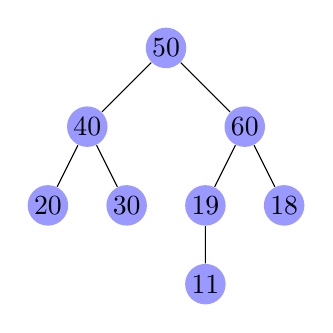
\begin{tikzpicture}
[level distance = 10mm,
every node/.style = {fill=blue!40,circle,inner sep=1pt},
level 1/.style = {sibling distance = 20mm,nodes ={fill = blue!40}},
level 2/.style = {sibling distance = 10mm,nodes = {fill = blue!40}},
level 3/.style = {sibling distance = 5mm , nodes = {fill = blue!40}}]
\node {50}
child {node{40}
child{node{20}}
child{node{30}}
}
child{node{60}
child{node{19}
child{node{11}}
}
child{node{18}}
};


\end{tikzpicture}
\end{document}